\documentclass[12pt,a4paper]{scrartcl}
\usepackage[utf8]{inputenc}
\usepackage[english,russian]{babel}
\usepackage{amssymb,amsfonts}
\usepackage{amsmath,cite,enumerate}
\usepackage{float,indentfirst}
\usepackage{graphicx}
\usepackage{geometry} % Меняем поля страницы
\geometry{left=2cm}% левое поле
\geometry{right=1.5cm}% правое поле
\geometry{top=1cm}% верхнее поле
\geometry{bottom=2cm}% нижнее поле
\graphicspath{{images/}}

\begin{document}


\begin{titlepage}
  \begin{center}
    Санкт-Петербургский Политехнический Университет     Петра Великого \\
    
    Институт компьютерных наук и технологий \\
    
    Кафедра компьютерных систем и программных технологий
  \end{center}
  
  \vfill
  
  \begin{center}
  Лабораторная работа №4 и №5\\
  по теме\\
  "Аналоговая, частотная и фазовая модуляции"\\
\end{center}

\vfill

\newlength{\ML}
\settowidth{\ML}{«\underline{\hspace{0.7cm}}» \underline{\hspace{2cm}}}
\hfill\begin{minipage}{0.4\textwidth}
  Выполнил студент группы 33501/3\\
  \underline{\hspace{\ML}} Кисличенко Б.\,Д\\
\end{minipage}%

\bigskip

\settowidth{\ML}{«\underline{\hspace{0.7cm}}» \underline{\hspace{2cm}}}
\hfill\begin{minipage}{0.4\textwidth}
  Руководитель\\
  \underline{\hspace{\ML}} Богач Н.\,В\\
\end{minipage}%

\vfill
 
\begin{center}
  Санкт-Петербург\\
2018 
\end{center}

\end{titlepage}

\section{Цель}
\label{sec:goal}

Изучение амплитудной, частотной и фазовой модуляции/демодуляции.\\

\section{Постановка задачи}
\label{sec:task}

1) Сгенерировать однотональный сигнал низкой частоты.

2) Выполнить амплитудную модуляцию (АМ) сигнала по закону $$u(t)=(1+MU_m cos(\Omega t))cos(\omega_0 t+\phi_0)$$ для различных значений глубины модуляции М. Использовать встроенную функцию MatLab ammod.

3) Получить спектр модулированного сигнала.

4) Выполнить модуляцию с подавлением несущей  $$u(t)=MU_m cos(\Omega t))cos(\omega_0 t+\phi_0)$$ Получить спектр.

5) Выполнить однополосную модуляцию:

$$u(t)=U_m cos(\Omega t)cos(\omega_0 t+\phi_0) + \frac{U_m}{2} \sum_{n=1}^N M_n (cos(\omega_0+\Omega_n)t+\phi_0+\Phi_n)$$
положив n=1.

6) Выполнить синхронное детектирование и получить исходный однополосный сигнал.

7) Расчитать КПД модуляции. $$\eta_A M = \frac{U_m^2 M^2/4}{P_U} = \frac{M^2}{M^2+1}$$

8) Сгенерировать однотональный сигнал низкой частоты.

9) Выполнить фазовую модуляцию/демодуляцию сигнала по закону $u(t) = (U_m cos(\Omega t+ks(t))$, используя встроенную функцию MatLab pmmod, pmdemod

10) Получить спектр модулированного сигнала.

11) Выполнить частотную модуляцию/демодуляцию по закону $$u(t) = (U_m cos(\omega_0 t+k\int_o^t s(t)dt+\varpi_0)$$ исаользуя встроенные функции MatLab fmmod, fmdemod.

\clearpage
\newpage

\section{Модуляция/Демодуляция}
\label{sec:teoriya}

Как правило, информационные сигналы являются низкочастотными и ограниченными по ширине спектра, тогда как методы передачи сигналов рассчитаны на работу с высокочастотным сигналом. Перенос спектра сигналов из низкочастотной области на заданную частоту, т.е. в выделенную для их передачи область высоких частот выполняется операцией модуляции.

$s(t)$ - низкочастотный сигнал, подлежащий передаче по какому-либо каналу связи. В канале связи для передачи данного сигнала выделяется определенный диапазон высоких частот и формируется вспомогательный периодический высокочастотный сигнал $u(t) = f(t; a_1, a_2, … a_m).$ Совокупность параметров $a_i$ определяет форму вспомогательного сигнала. Значения параметров $a_i$ в отсутствие модуляции являются величинами постоянными.

Если на один из этих параметров перенести сигнал s(t), т.е. сделать его значение пропорционально зависимым от значения s(t) во времени (или по любой другой независимой переменной), то форма сигнала u(t) приобретает новое свойство. Она служит для переноса информации, содержащейся в сигнале s(t). Сигнал u(t) называется \textbf{несущим сигналом}, \textbf{несущим колебанием} или просто \textbf{несущей}, а физический процесс переноса информации на параметры несущего сигнала – его \textbf{модуляцией}. Исходный информационный сигнал s(t) называют модулирующим, результат модуляции – \textbf{модулированным сигналом}. Обратную операцию выделения модулирующего сигнала из модулированного колебания называют \textbf{демодуляцией} или д\textbf{етектированием}.

Наиболее распространенной формой несущих сигналов являются гармонические колебания:
$$u(t)=Ucos(\omega t+\phi),$$

которые имеют три свободных параметра: U, $\omega$ и $\phi$. В зависимости от того, на какой из данных параметров переносится информация, различают \textbf{амплитудную (АМ)}, \textbf{частотную (ЧМ)} или \textbf{фазовую (ФМ)} модуляцию несущего сигнала.

При использовании в качестве несущих сигналов периодических последовательностей импульсов (например, прямоугольных) свободными параметрами модуляции могут быть амплитуда, длительность, частота следования и фаза (положение импульса относительно тактовой точки) импульсов. Таким образом, существует четыре основных вида импульсной модуляции: АИМ, ЧИМ и ФИМ.

\subsection{Амплитудная модуляция}
\label{sec:AM}

В настоящее время АМ применяется в основном только для радиовещания на сравнительно низких частотах и для передачи изображения в телевизионном вещании. Это вызвано низким КПД использования энергии модулированных сигналов.

При АМ выполняется перенос информации s(t) => U(t) при постоянных значениях параметров несущей частоты $\omega$ и $\phi$. АМ – сигнал представляет собой произведение информационной огибающей U(t) и гармонического колебания ее заполнения с более высокими частотами: $$U(t)=U_m[1+Ms(t)],$$ где $U_m$ - постоянная амплитуда несущего колебания при отсутсвии входного (модулирующего) сигнала s(t), M - глубина АМ.

Если модулирующий сигнал представлен одночастотным гармоническим колебанием с амплитудой $S_0$, то коэффициент модуляции равен отношению амплитуд модулирующего и несущего колебания $М=S_0/U_m$. Значение М должно находиться в пределах от 0 до 1 для всех гармоник модулирующего сигнала. При значении М<1 форма огибающей несущего колебания полностью повторяет форму модулирующего сигнала s(t)

Простейшая форма модулированного сигнала создается при однотональной амплитудной модуляции – модуляции несущего сигнала гармоническим колебанием с одной частотой $\Omega$: $$u(t)=U_m[1+Mcos(\Omega t)]cos(\omega_0 t)$$

Основная теорема модуляции:$$u(t)=U_m cos(\omega_0 t) + \frac{U_m M}{2} cos[(\omega_0 + \Omega)t] + \frac{U_m M}{2} cos[(\omega_0 - \Omega)t].$$

Модулирующее колебание с частотой $\Omega$ перемещается в область частоты $\omega_0$ и расщепляется на два колебания, симметричные относительно частоты $\omega_0$, с частотами соответственно $(omega_0 + \Omega)$ - верхняя боковая частота, и $(omega_0 - \Omega)$ - нижняя боковая частота. Физическая ширина спектра модулированного сигнала в два раза больше ширины спектра сигнала модуляции.  

КПД АМ: $$\eta_{AM}=\frac{U_m^2 M^2 /4}{P_U} = \frac{M^2}{M^2+2}.$$
 
Отсюда следует, что при М=1 КПД амплитудной модуляции составляет только 33$%$, а на практике обычно меньше 20$%$.

При идентичности информации в группах верхних и нижних боковых частот нет необходимости в их одновременной передаче. Одна из них перед подачей сигнала в канал связи может быть удалена, чем достигается двукратное сокращение полосы занимаемых сигналом частот.

Для верхней или нижней боковой полосы:
$$u(t)=U_m cos(\Omega t)cos(\omega_0 t+\phi_0) + \frac{U_m}{2} \sum_{n=1}^N M_n (cos(\omega_0 \pm \Omega_n)t \pm \phi_0 \pm \Phi_n)$$

Внешняя форма ОБП-сигнала сходна с обычным АМ-сигналом, но ее огибающая имеет в два раза меньшую амплитуду по сравнению с АМ при М = 1.

%Рисунок 1
\begin{figure}[h!]
\center{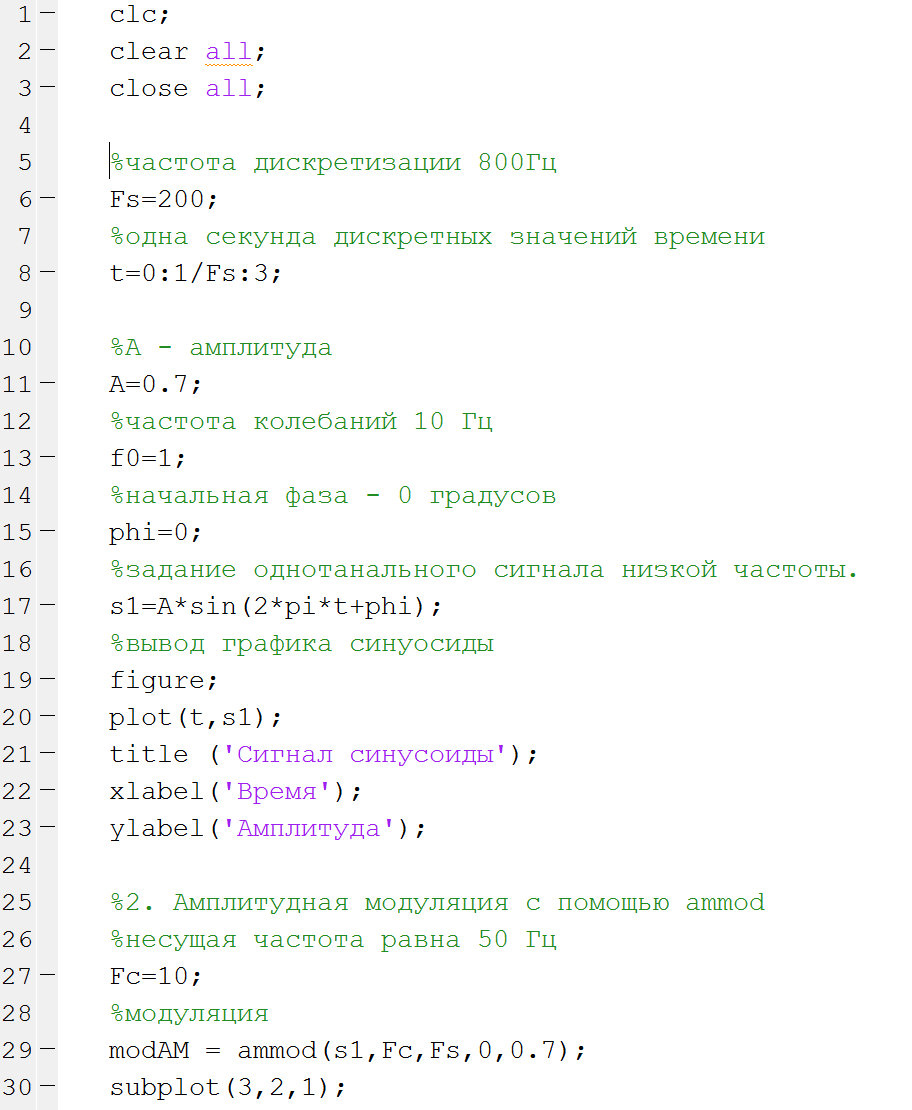
\includegraphics[width=0.75\linewidth]{am1}}
\caption{Код Matlab (часть 1)}
\end{figure}

%Рисунок 2
\begin{figure}[h!]
\center{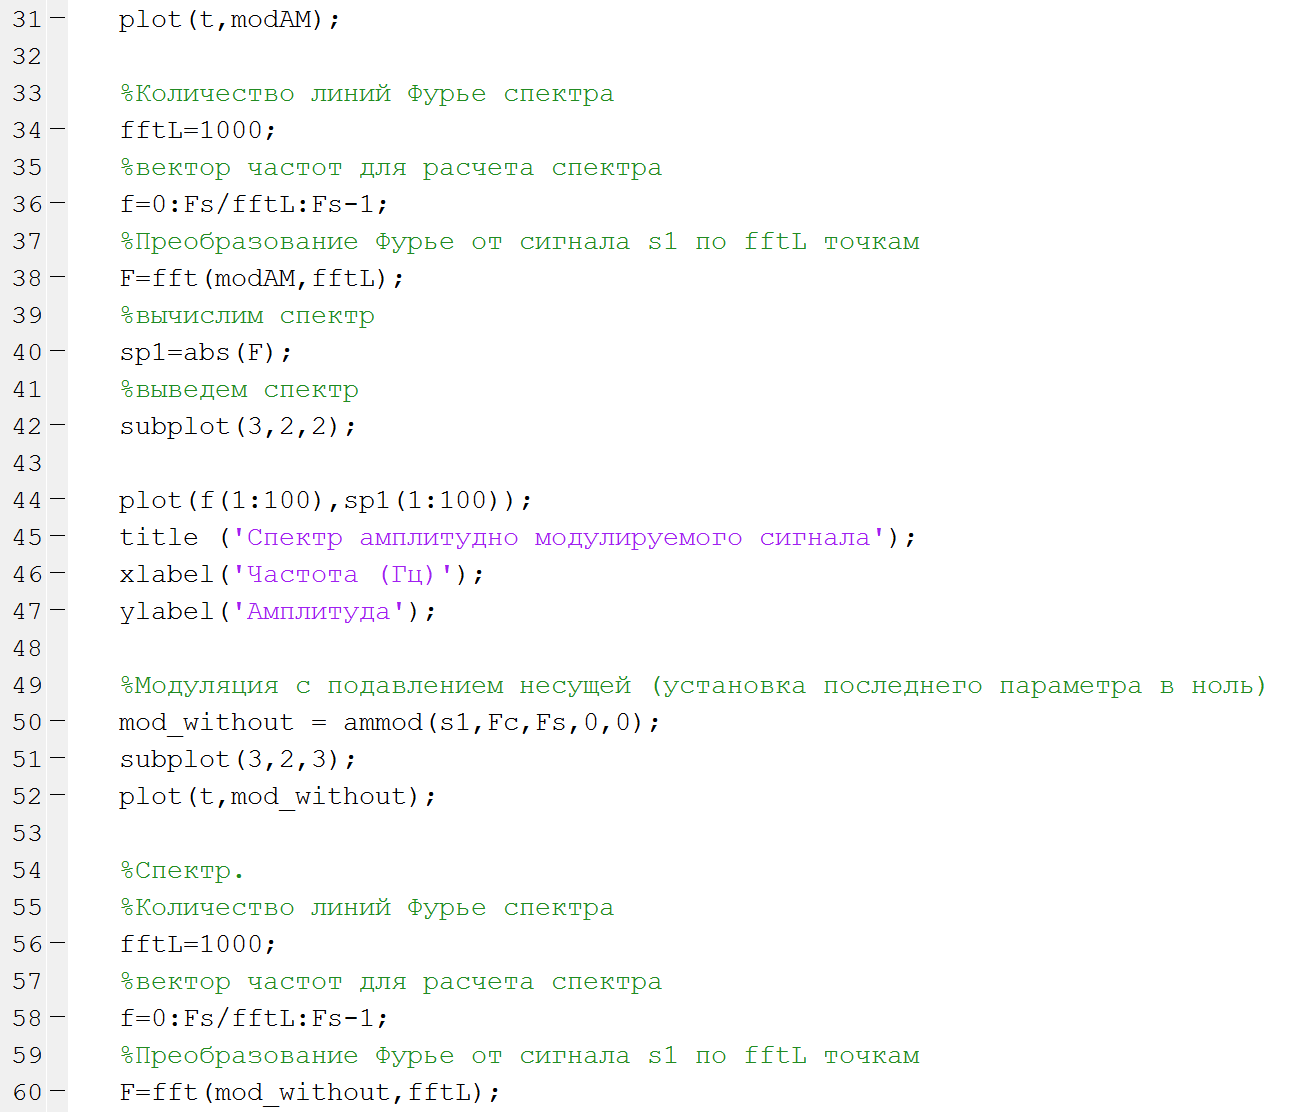
\includegraphics[width=0.75\linewidth]{am2}}
\caption{Код Matlab (часть 2)}
\end{figure}

%Рисунок 3
\begin{figure}[h!]
\center{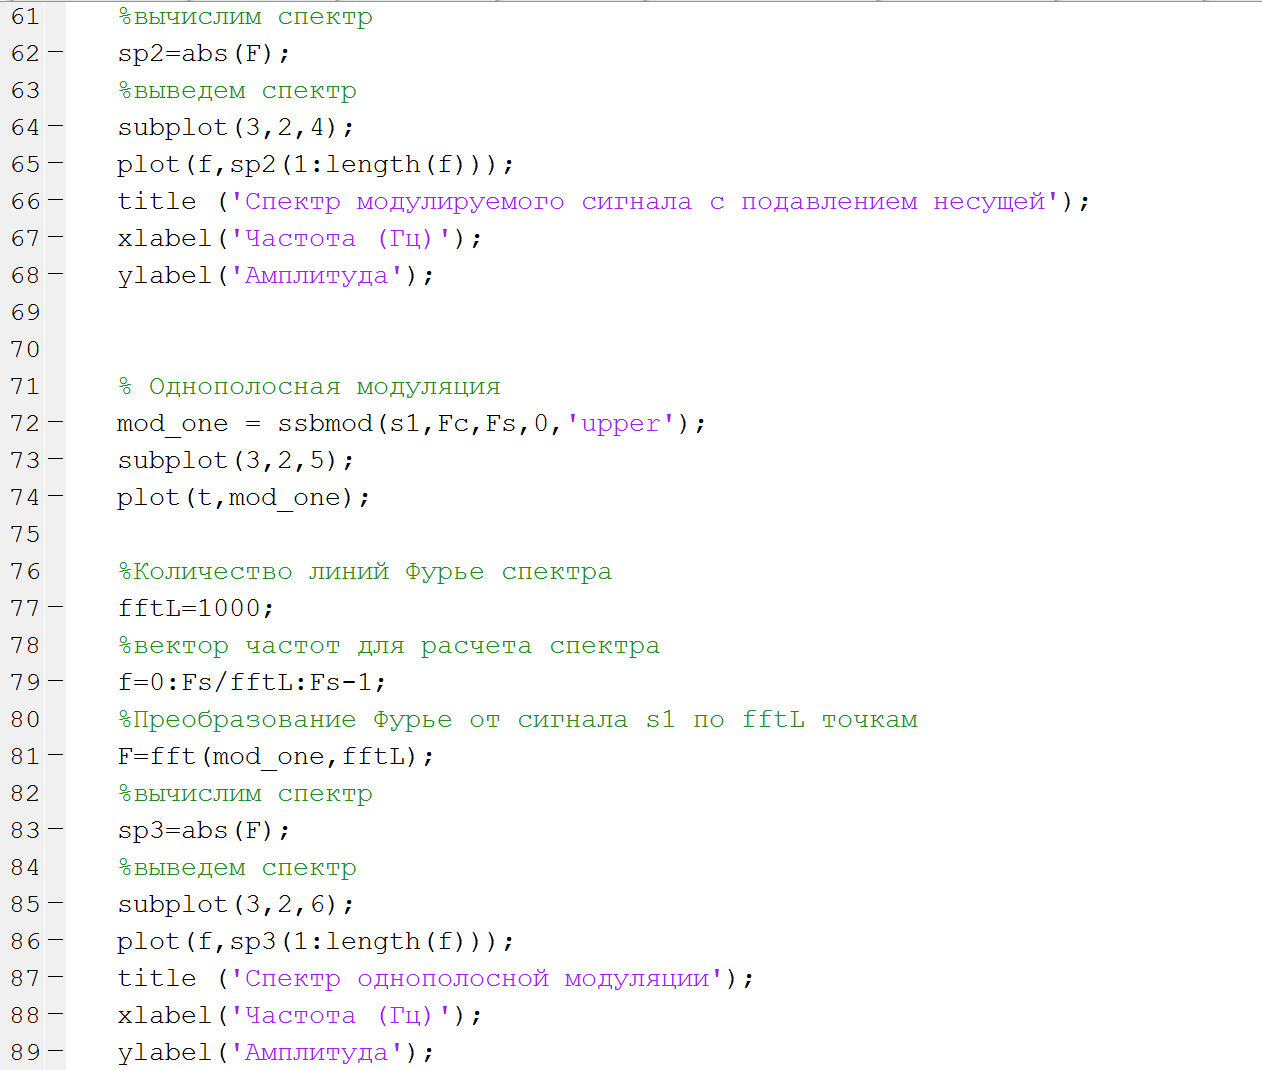
\includegraphics[width=0.75\linewidth]{am3}}
\caption{Код Matlab (часть 3)}
\end{figure}

%Рисунок 4
\begin{figure}[h!]
\center{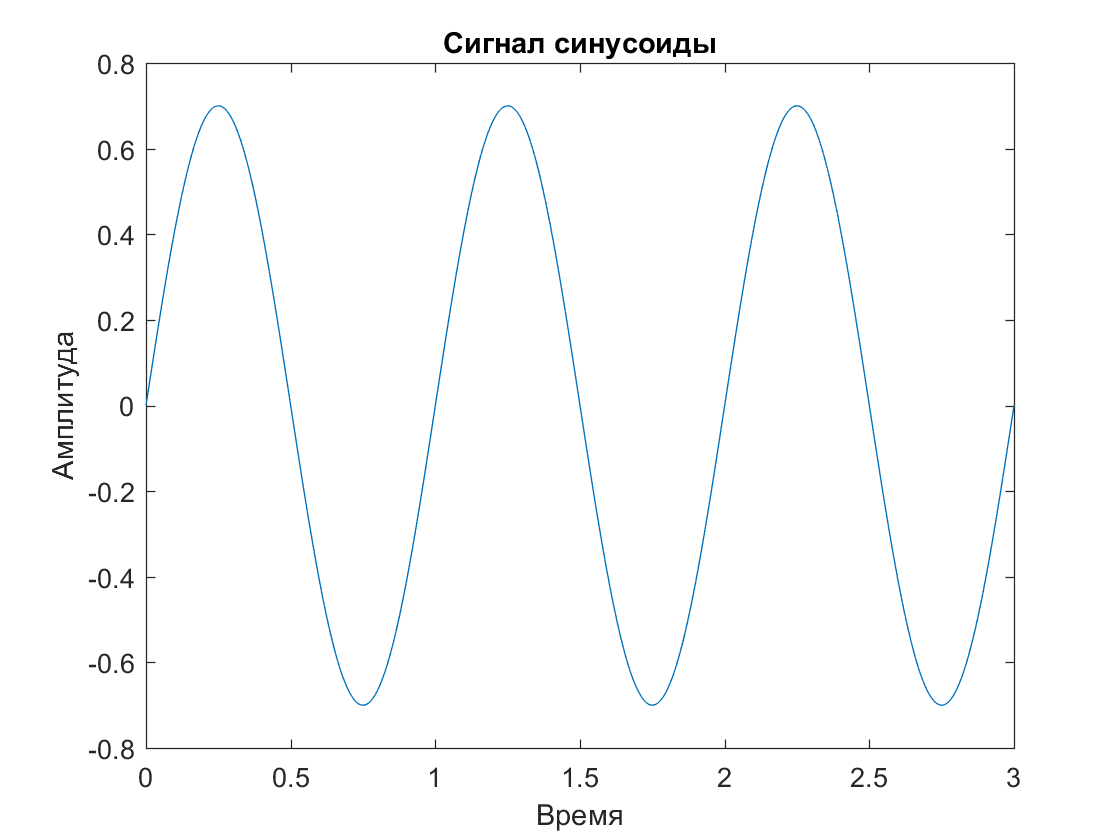
\includegraphics[width=0.6\linewidth]{sin}}
\caption{Однотональная синусоида}
\end{figure}

%Рисунок 5
\begin{figure}[h!]
\center{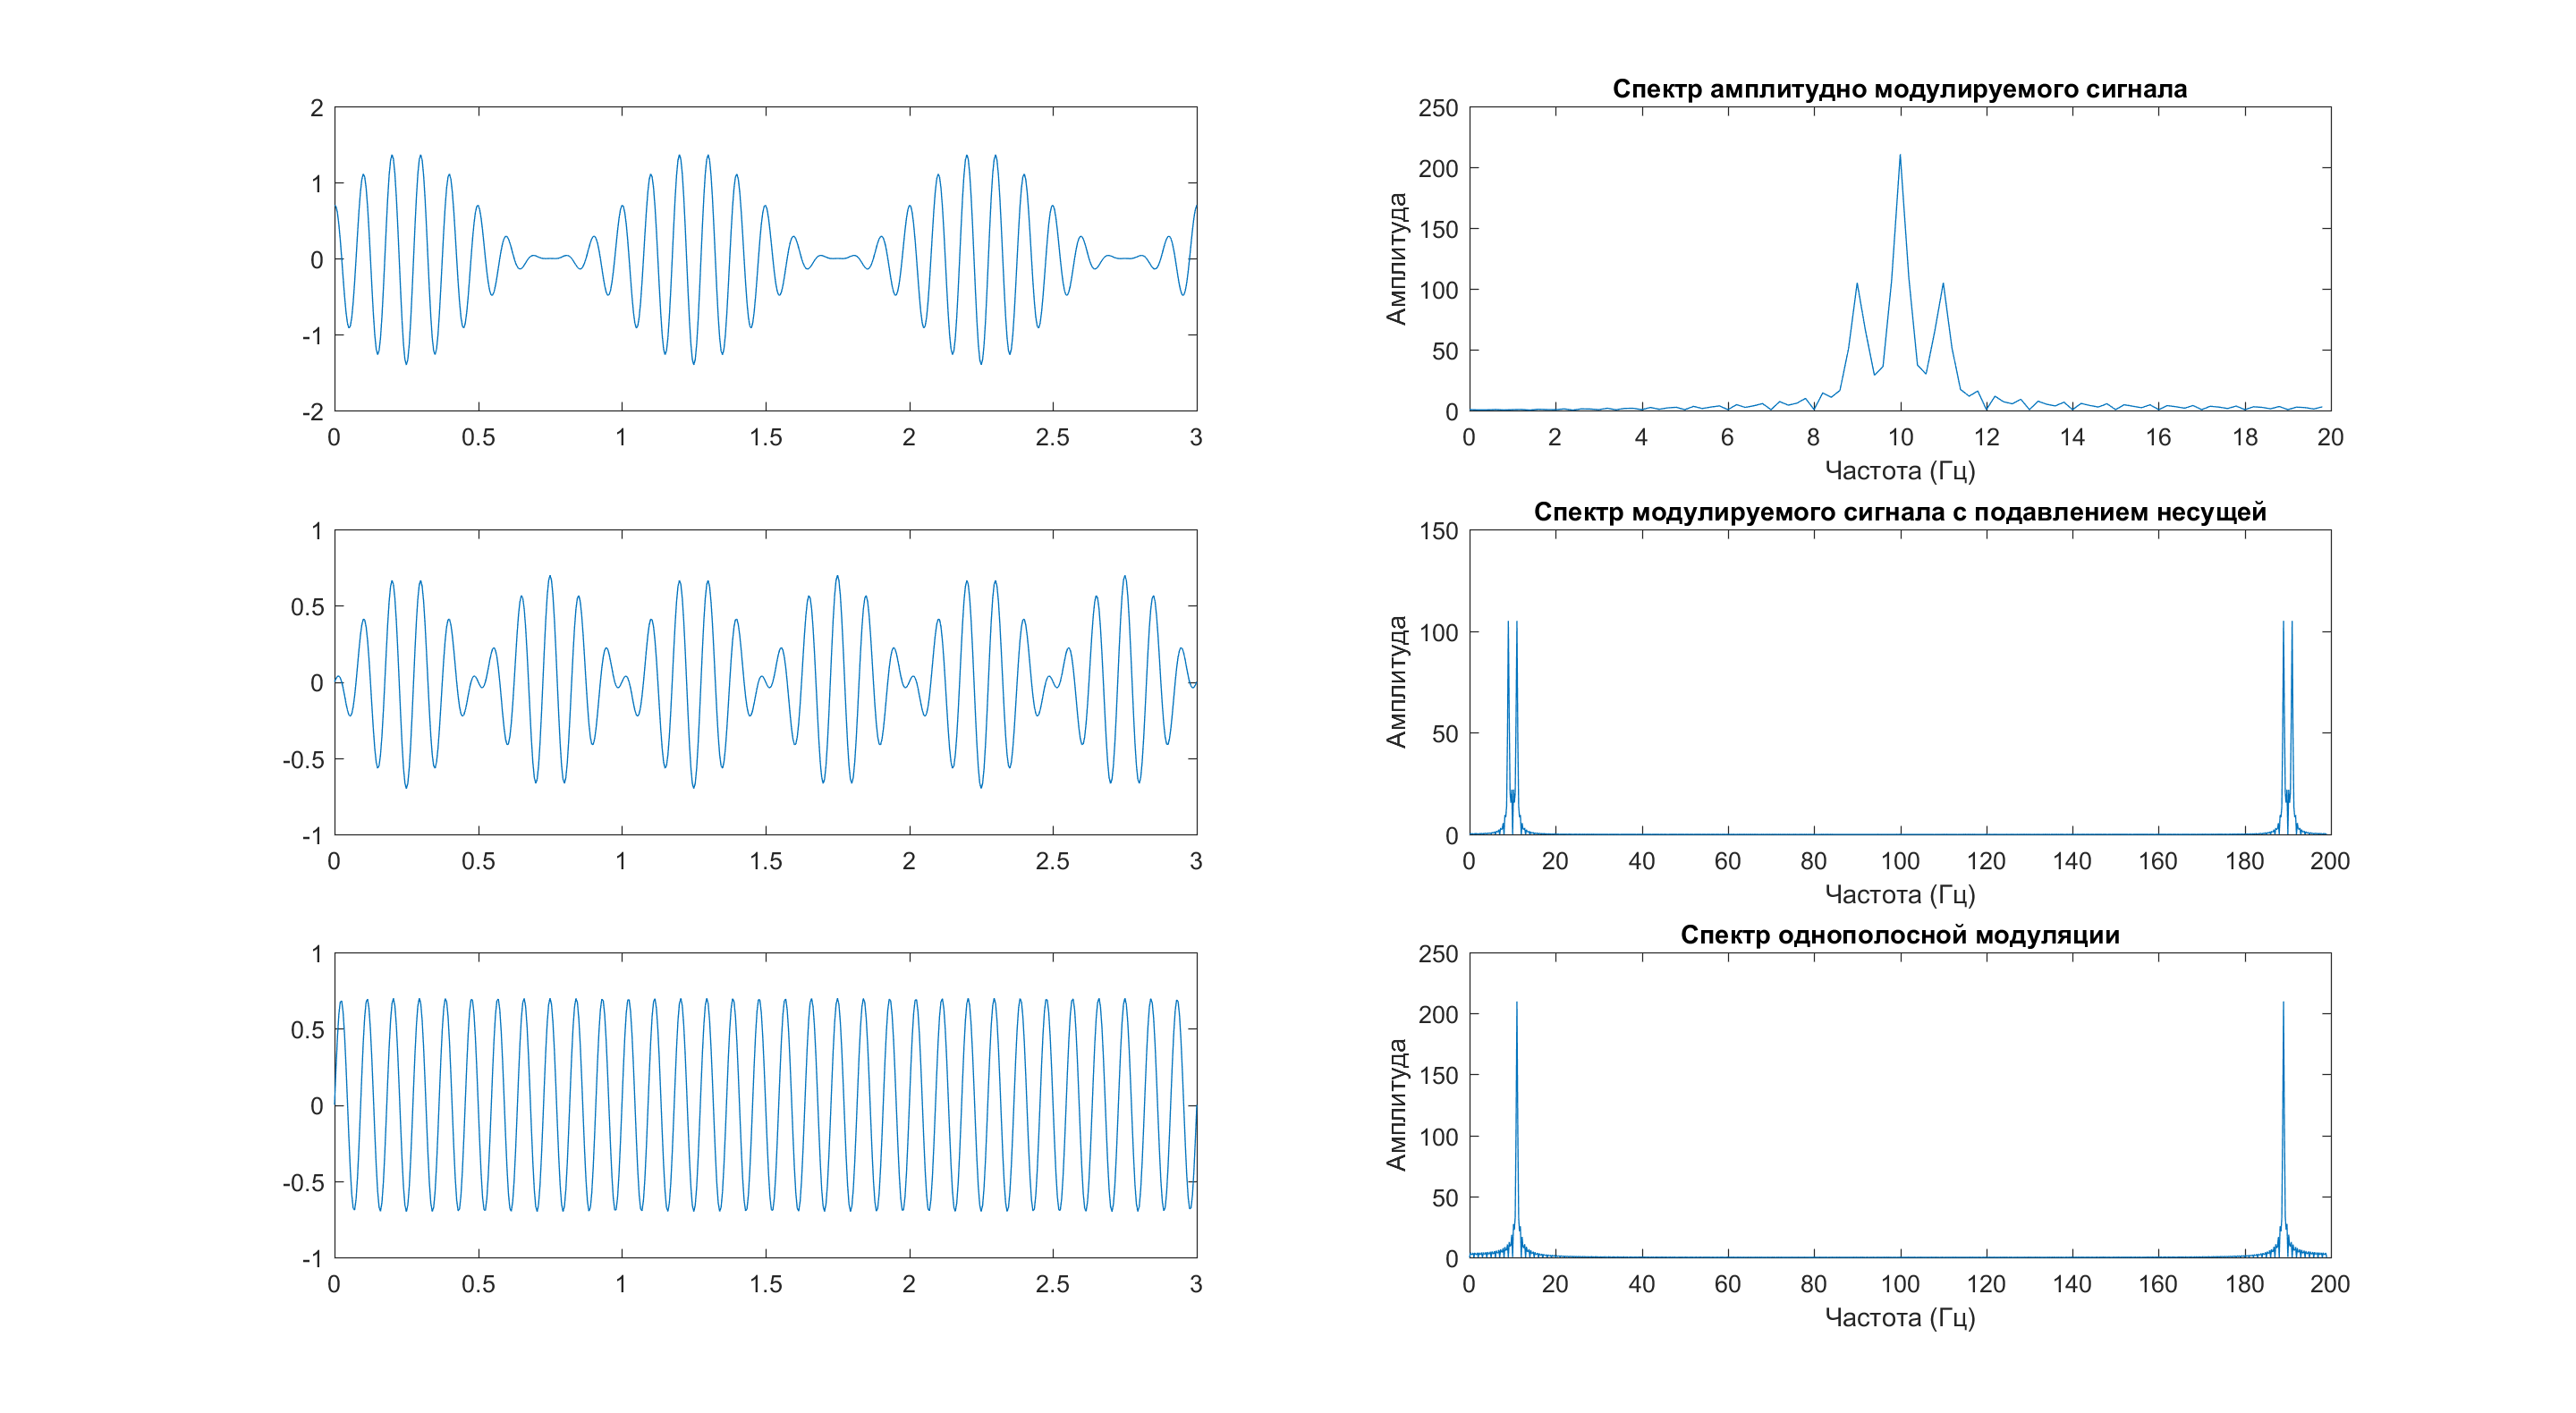
\includegraphics[width=1\linewidth]{am_sp}}
\caption{Модуляции и спектры}
\end{figure}

\clearpage
\newpage

\subsection{Синхронное детектирование}
\label{sec:syn_demod}

При синхронном детектировании модулированный сигнал умножается на опорное колебание с частотой несущего колебания. Без учета начальных фаз колебаний: $$y(t)=u(t)cos \omega_0 t cos \omega_0 t = \frac{1}{2}U(t)+\frac{1}/{2} U(t) cos 2 \omega_0 t.$$

сигнал разделяется на два слагаемых, первое из которых повторяет исходный модулирующий сигнал, а второе повторяет модулированный сигнал на удвоенной несущей частоте $2 \omega_0$. Форма новой несущей при синхронном детектировании является чистой гармоникой, в отличие от двухполупериодного детектирования, где новая несущая содержит дополнительные гармоники более высоких частот. Физический амплитудный спектр сигналов после демодуляции подобен спектру двухполупериодного детектирования, но однозначно соотносится со спектром входного модулированного сигнала: амплитуды гармоник модулированного сигнала на частоте $2 \omega_0$ в два раза меньше амплитуд входного сигнала, постоянная составляющая равна амплитуде несущей частоты $\omega_0$ и не зависит от глубины модуляции, амплитуда информационного демодулированного сигнала в два раза меньше амплитуды исходного модулирующего сигнала. Особенностью синхронного детектирования является независимость от глубины модуляции, т.е. коэффициент модуляции сигнала может быть больше единицы.

\begin{figure}[h!]
\center{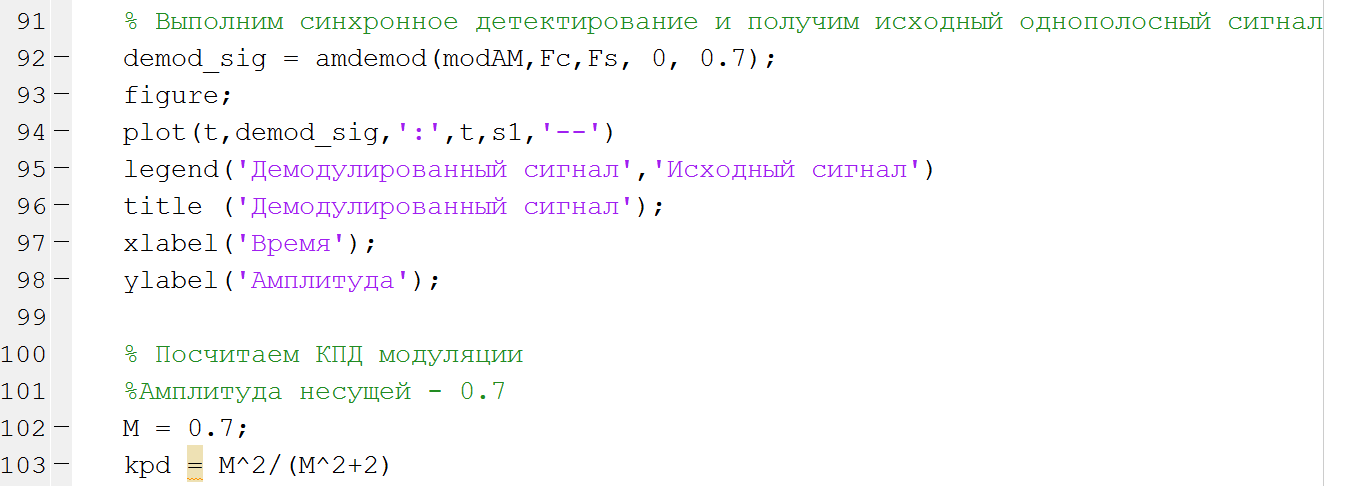
\includegraphics[width=0.75\linewidth]{ad1}}
\caption{Код демодуляции}
\end{figure}

%Рисунок 7
\begin{figure}[h!]
\center{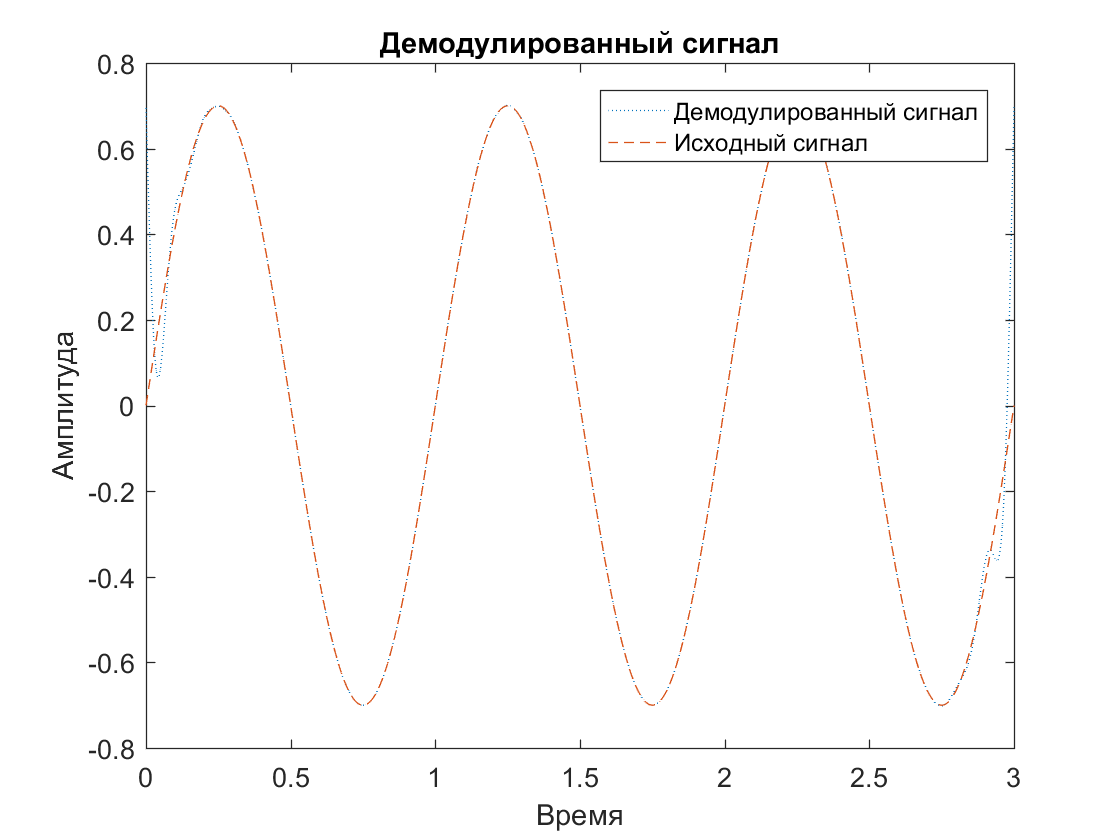
\includegraphics[width=0.6\linewidth]{ad}}
\caption{Демодуляция}
\end{figure}

\clearpage
\newpage
\subsection{Фазовая модуляция}
\label{sec:FM}
При фазовой модуляции значение фазового угла постоянной несущей частоты колебаний $\omega_0$ пропорционально амплитуде модулирующего сигнала s(t). Соответственно, уравнение ФМ-сигнала определяется выражением:
$$u(t) = U_m cos[\omega_0 t+k*s(t)],$$ где k - коэфициент пропорциональности.

При s(t) = 0, ФМ-сигнал является простым гармоническим колебанием. С увеличением значений s(t) полная фаза колебаний $\verphi(t)=\omega_0t + k*s(t)$ нарастает во времени быстрее и опережает линейное нарастание $\omega_0 t$. Соответственно, при уменьшении значений s(t) скорость роста полной фазы во времени спадает. В моменты экстремальных значений s(t) абсолютное значение фазового сдвига $\delta \verphi $между ФМ-сигналом и значением $\omega t$ немодулированного колебания также является максимальным и носит название девиации фазы (вверх $\delta \phi_в = k*s_{max}(t)$, или вниз $\delta \phi_н = k*s_{min}(t)$ с учетом знака экстремальных значений модулирующего сигнала).


%Рисунок 1
\begin{figure}[h!]
\center{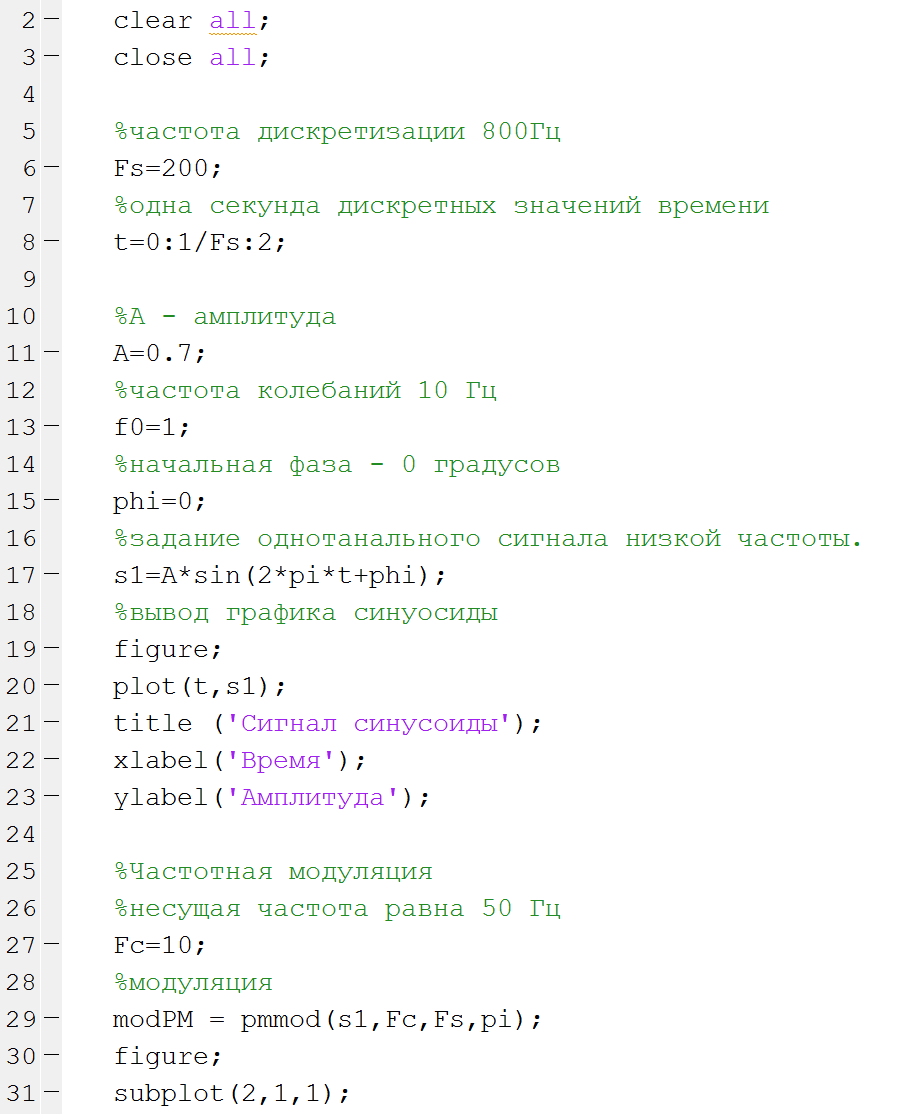
\includegraphics[width=0.6\linewidth]{sin_code2}}
\caption{Код Matlab для фазовой модуляции(часть 1)}
\end{figure}

%Рисунок 2
\begin{figure}[h!]
\center{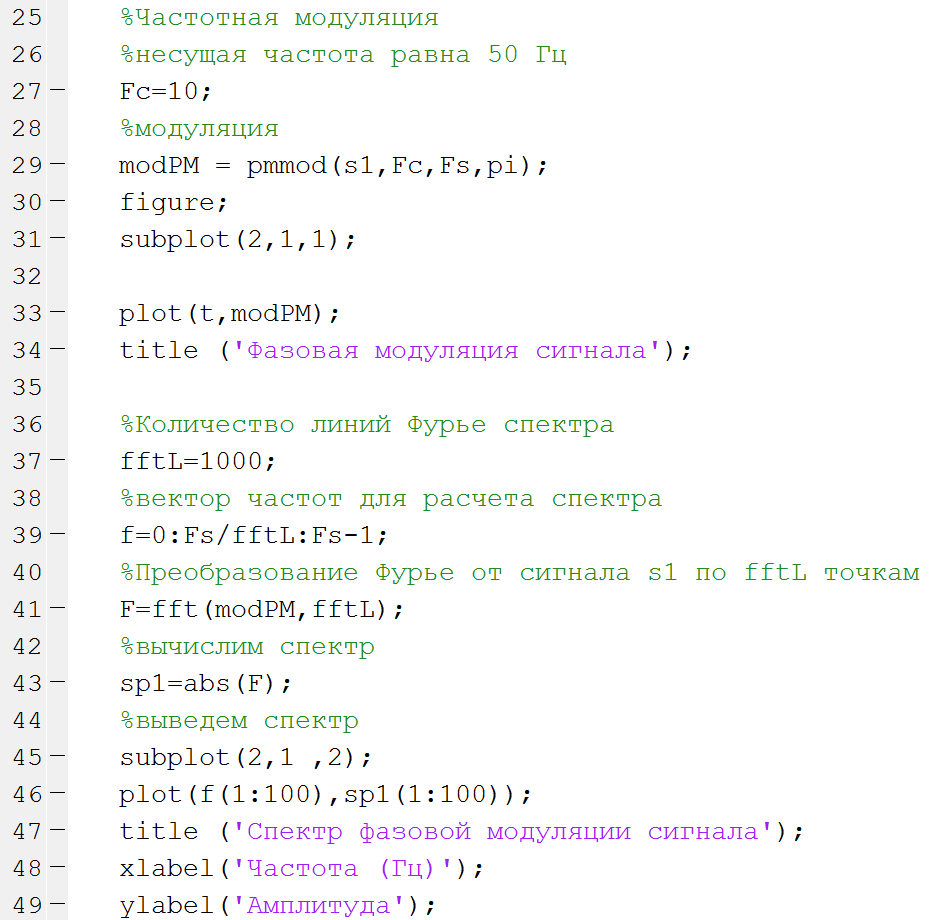
\includegraphics[width=0.6\linewidth]{pm1}}
\caption{Код Matlab для фазовой модуляции(часть 2)}
\end{figure}

%Рисунок 4
\begin{figure}[h!]
\center{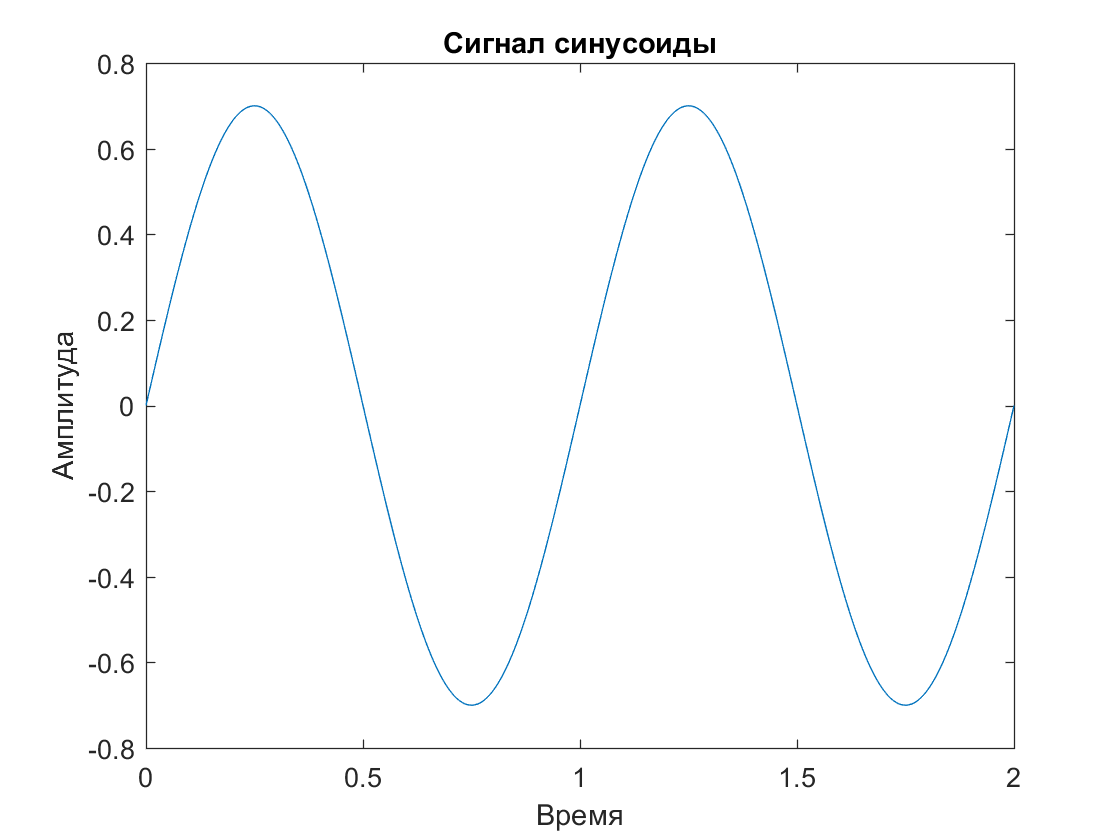
\includegraphics[width=0.6\linewidth]{sin2}}
\caption{Однотональная синусоида}
\end{figure}

%Рисунок 3
\begin{figure}[h!]
\center{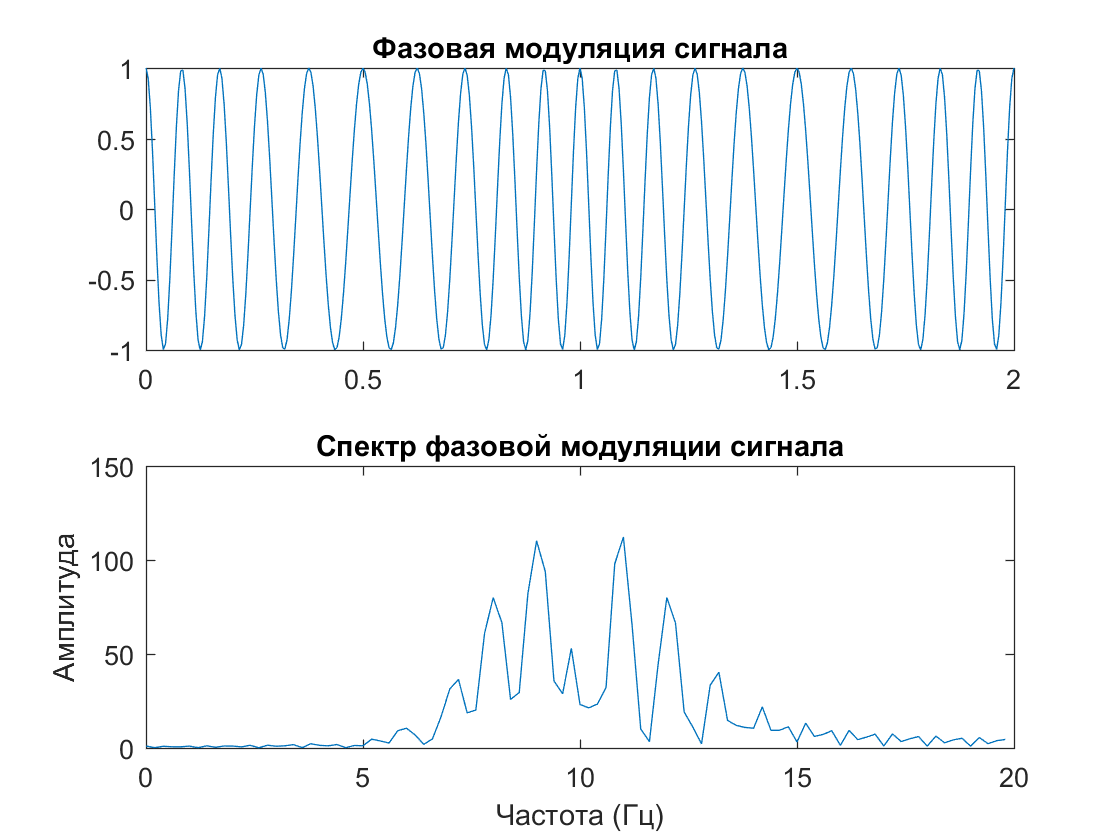
\includegraphics[width=0.75\linewidth]{pm_mod}}
\caption{Фазовая модуляция}
\end{figure}

%Рисунок 3
\begin{figure}[h!]
\center{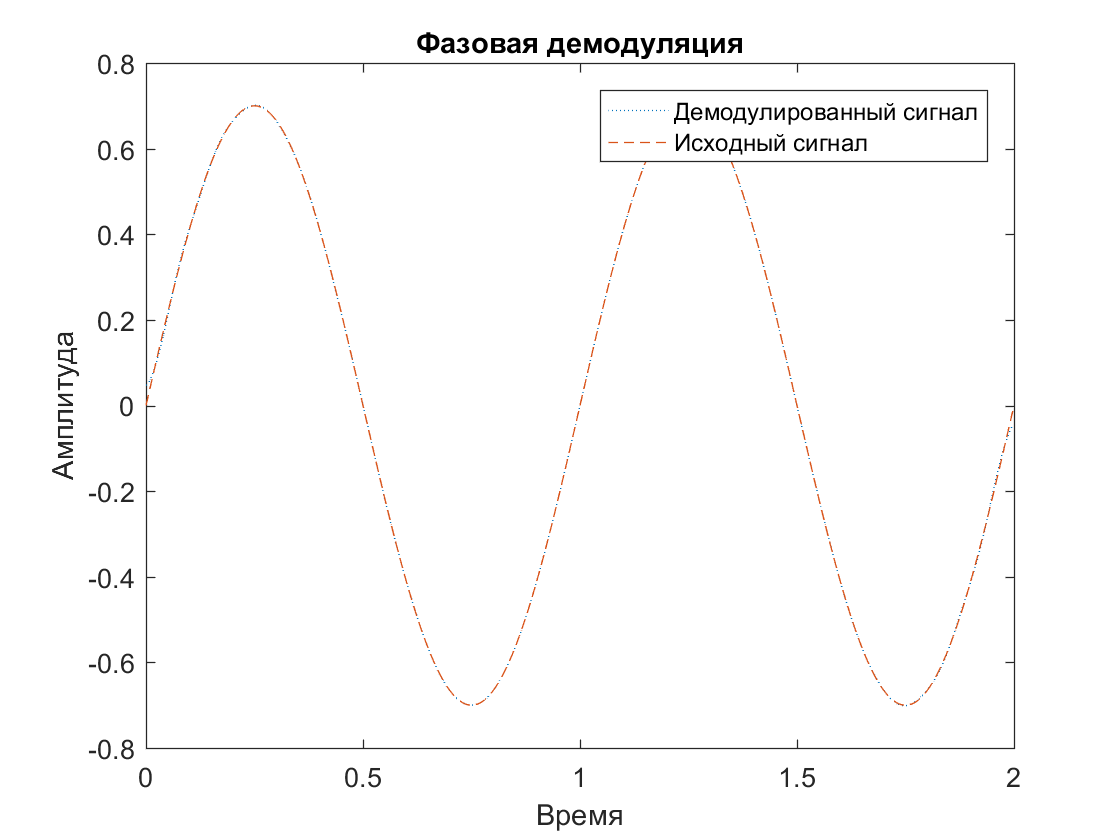
\includegraphics[width=0.75\linewidth]{pmk}}
\caption{Фазовая демодуляция}
\end{figure}


\clearpage
\newpage
\subsection{Частотная модуляция}
\label{sec:CHM}

Частотная модуляция характеризуется линейной связью модулирующего сигнала с мгновенной частотой колебаний, при которой мгновенная частота колебаний образуется сложением частоты высокочастотного несущего колебания $omega_0$ со значением амплитуды модулирующего сигнала с определенным коэффициентом пропорциональности k: $$\omega(t)=\omega_0 +k*s(t).$$
Соответственно, полная фаза колебаний:
$$\verphi(t)=\omega_0(t) + k \int_{-\infty}^t s(t)dt или \verphi(t)=\omega_0(t) + k \int_{-\infty}^t s(t)dt +\phi_0$$

Уравнение ЧМ-сигнала:

$$u(t)=U_m cos(\omega_0(t)+k\int_0^t s(t)dt +\phi_0)$$

Аналогично ФМ, для характеристики глубины частотной модуляции используются понятия девиации частоты вверх:
 $\delta \omega_в = k*s_{max}(t)$
 $и вниз \delta \omega_н = k*s_{min}(t)$ 


%Рисунок 1
\begin{figure}[h!]
\center{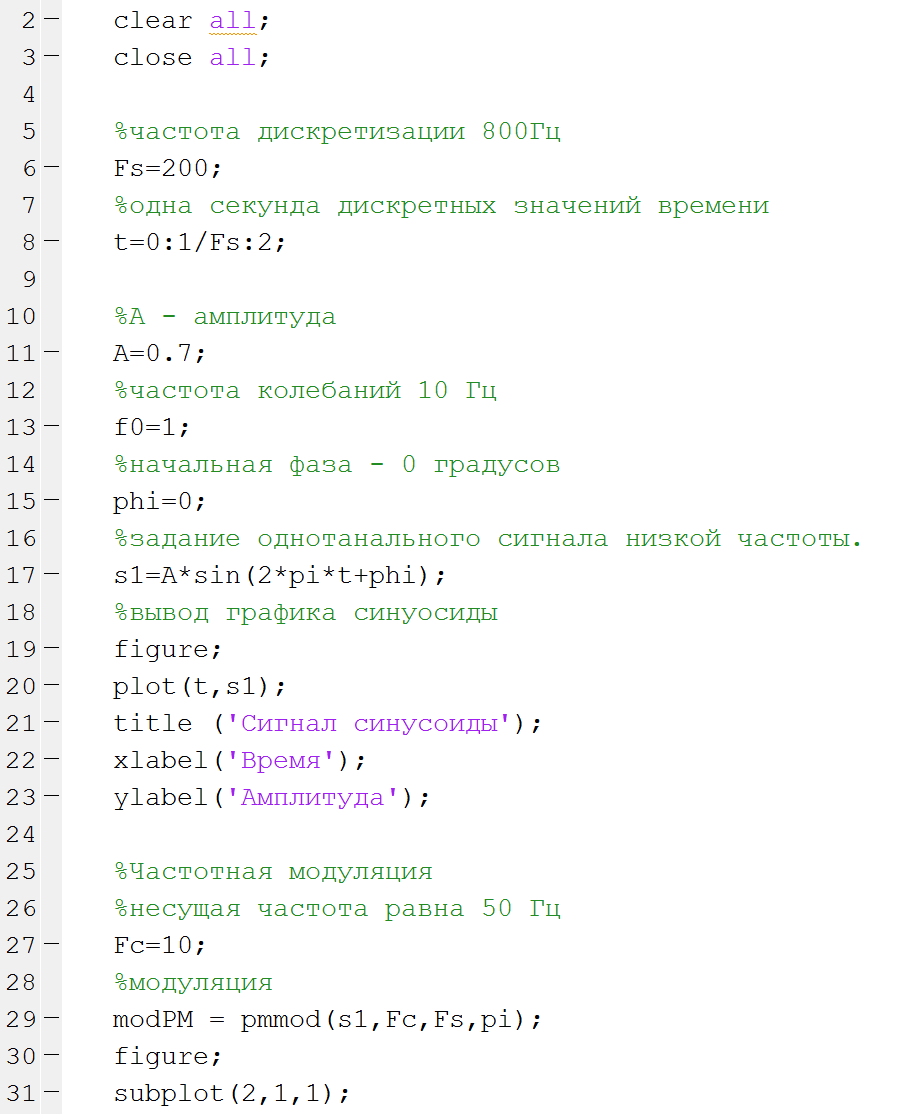
\includegraphics[width=0.6\linewidth]{sin_code2}}
\caption{Код Matlab для частотной модуляции(часть 1)}
\end{figure}

%Рисунок 2
\begin{figure}[h!]
\center{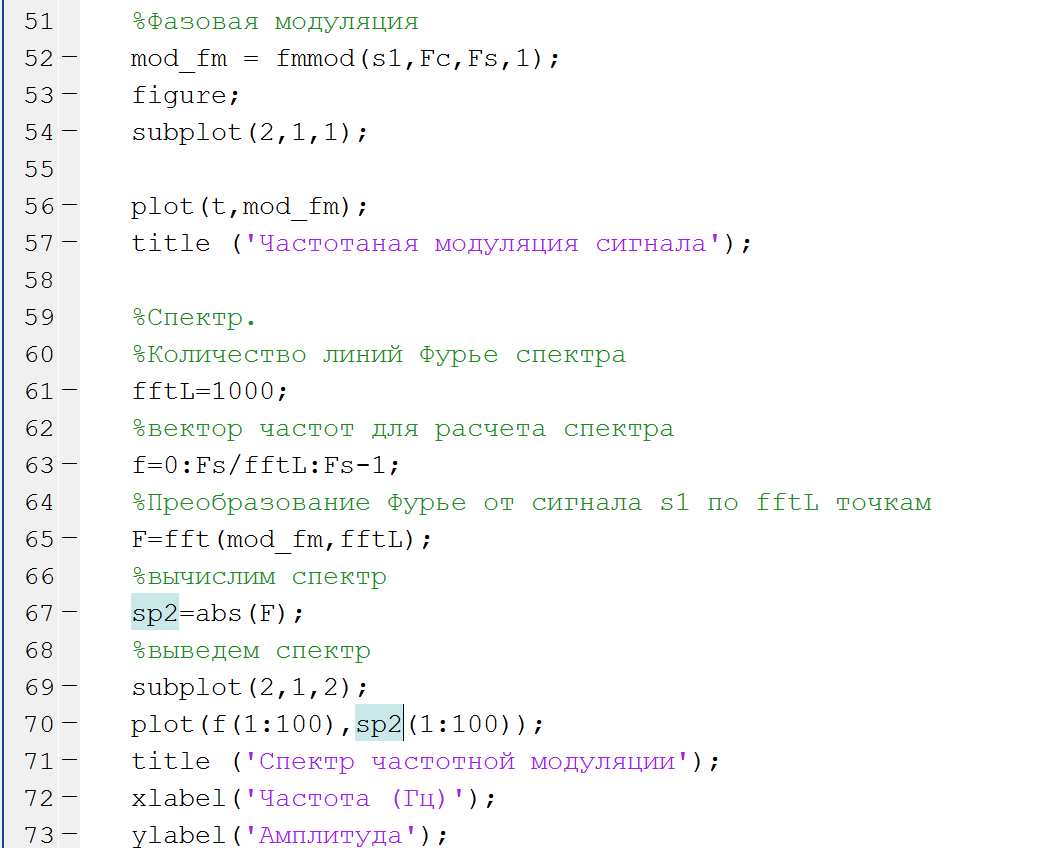
\includegraphics[width=0.6\linewidth]{fm1}}
\caption{Код Matlab для частотной модуляции(часть 2)}
\end{figure}

%Рисунок 4
\begin{figure}[h!]
\center{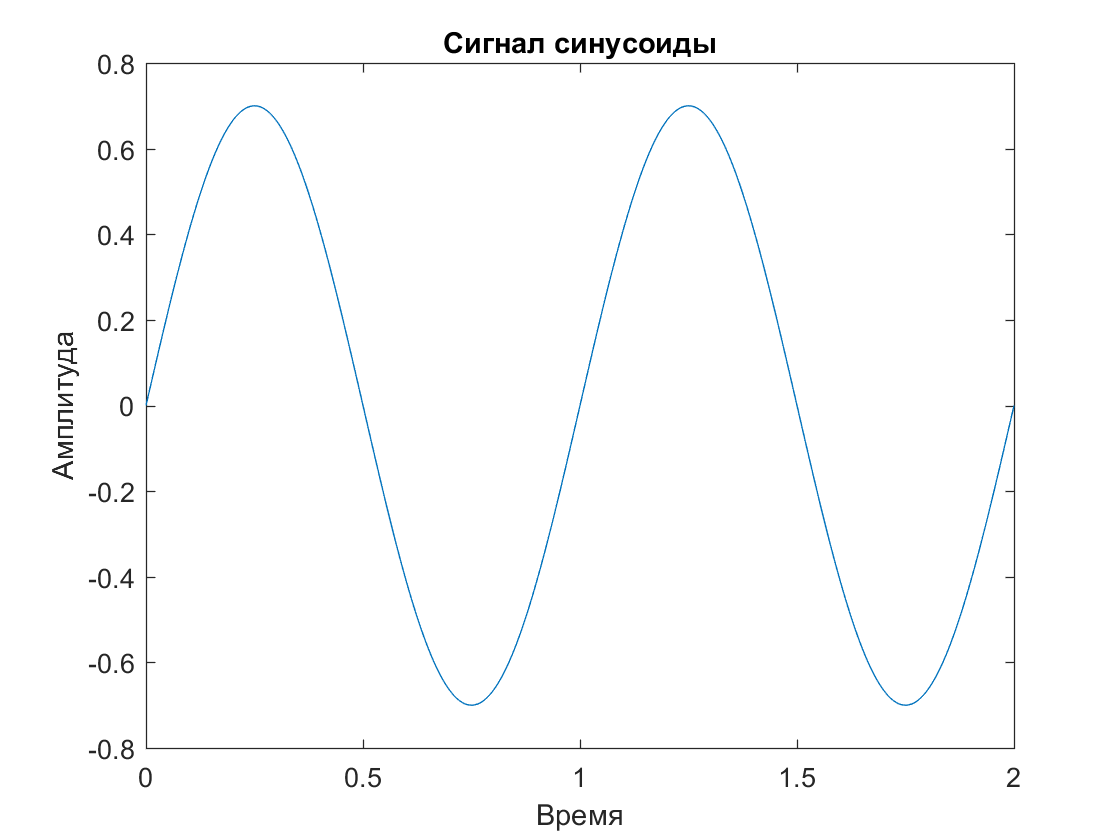
\includegraphics[width=0.6\linewidth]{sin2}}
\caption{Однотональная синусоида}
\end{figure}

%Рисунок 3
\begin{figure}[h!]
\center{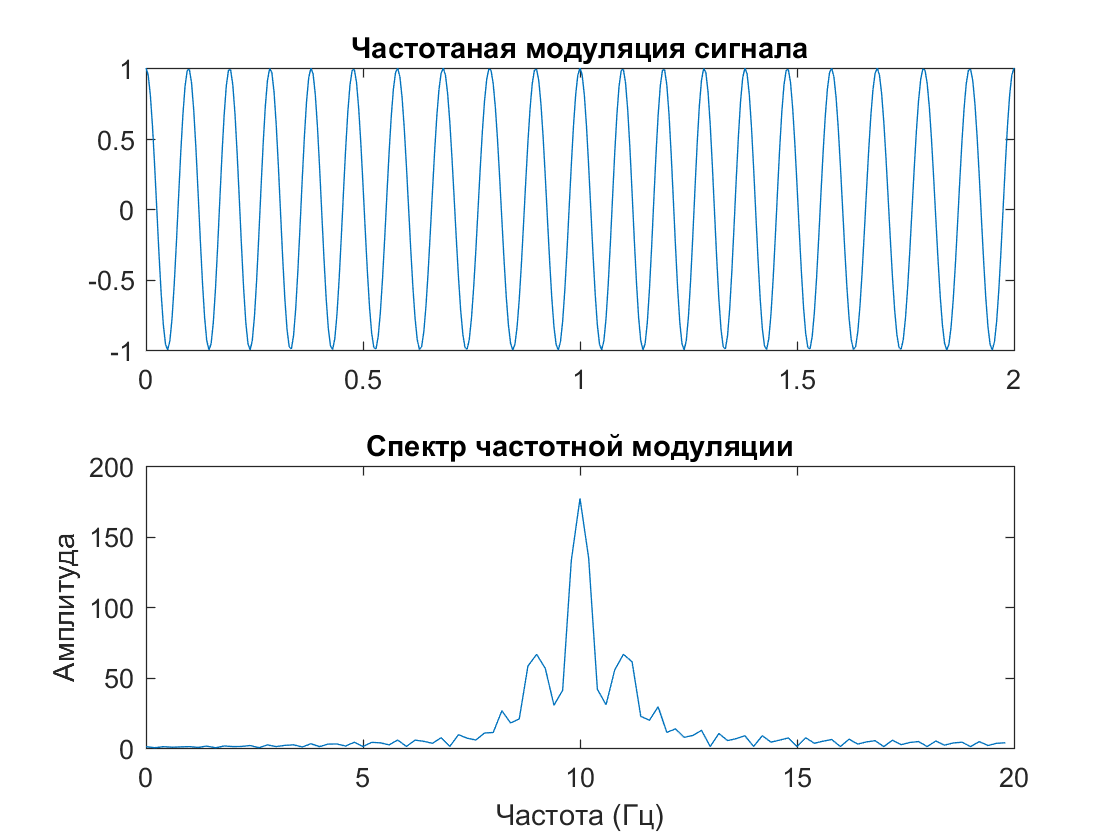
\includegraphics[width=0.75\linewidth]{fm_mod}}
\caption{Частотная модуляция}
\end{figure}

%Рисунок 3
\begin{figure}[h!]
\center{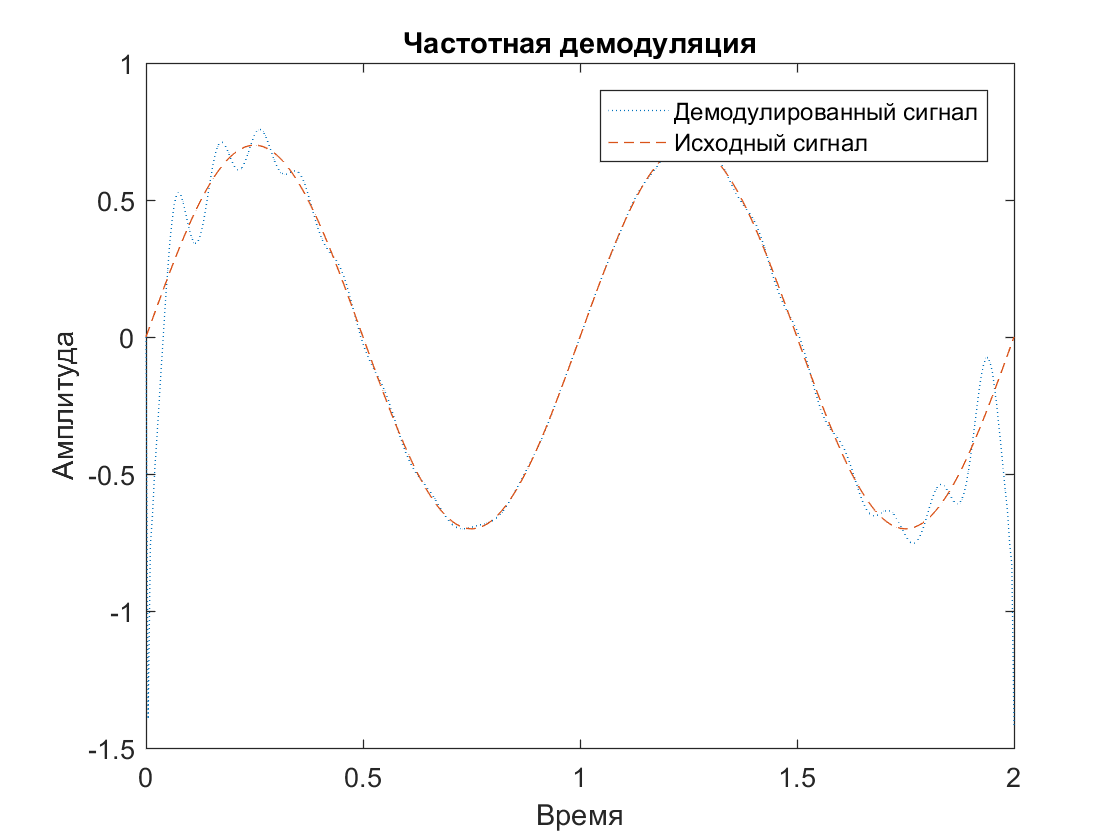
\includegraphics[width=0.75\linewidth]{fmk}}
\caption{Частотная демодуляция}
\end{figure}

\clearpage
\newpage

\section{Вывод}
\label{sec:afterWork}

 Основными достоинствами \textbf{амплитудной модуляции} являются:

 \begin{itemize}
    \item  узкая ширина спектра АМ сигнала;
    \item  простота получения модулированных сигналов.
 \end{itemize}
    
Недостатками этой модуляции являются:

\begin{itemize}
    \item   низкая помехоустойчивость (т. к. при воздействии помехи на сигнал искажается его форма — огибающая, которая и содержит передаваемое сообщение);
    \item  неэффективное использование мощности передатчика
 \end{itemize}
   
Амплитудная модуляция нашла широкое применение:

\begin{itemize}
    \item в системах телевизионного вещания (для передачи телевизионных сигналов);
    \item в системах звукового радиовещания и радиосвязи на длинных и средних волнах;
 \end{itemize}
 
 
  Достоинством ч\textbf{астотной модуляции} являются:

\begin{itemize}
\item высокая помехоустойчивость;
\item  более эффективное использование мощности передатчика;
\item  сравнительная простота получения модулированных сигналов.
\end{itemize}
    
Основным недостатком данной модуляции является большая ширина спектра модулированного сигнала.

Частотная модуляция используется:

\begin{itemize}
\item   в системах телевизионного вещания (для передачи сигналов звукового сопровождения);
\item   системах спутникового теле- и радиовещания;
\item  системах высококачественного стереофонического вещания (FM диапазон);
\item  радиорелейных линиях (РРЛ);
\item  сотовой телефонной связи.
\end{itemize}
  
Достоинствами \textbf{фазовой модуляции} являются:

\begin{itemize}
\item    высокая помехоустойчивость;
\item    более эффективное использование мощности передатчика.
\end{itemize}
   
Недостатками фазовой модуляции являются:

\begin{itemize}
\item  большая ширина спектра;
\item  сравнительная трудность получения модулированных сигналов и их детектирование 
\end{itemize}

\end{document}